\documentclass{article}

%% PAQUETES

% Paquetes generales
\usepackage[margin=2cm, paperwidth=210mm, paperheight=297mm]{geometry}
\usepackage[spanish]{babel}
\usepackage[utf8]{inputenc}
\usepackage{gensymb}

% Paquetes para estilos
\usepackage{textcomp}
\usepackage{setspace}
\usepackage{colortbl}
\usepackage{color}
\usepackage{color}
\usepackage{upquote}
\usepackage{xcolor}
\usepackage{listings}
\usepackage{caption}
\usepackage[T1]{fontenc}
\usepackage[scaled]{beramono}

% Paquetes extras
\usepackage{amssymb}
\usepackage{float}
\usepackage{graphicx}
\usepackage{array}
\usepackage{multirow}
\usepackage{amsmath}

%% Fin PAQUETES


% Definición de preferencias para la impresión de código fuente.
%% Colores
\definecolor{gray99}{gray}{.99}
\definecolor{gray95}{gray}{.95}
\definecolor{gray75}{gray}{.75}
\definecolor{gray50}{gray}{.50}
\definecolor{keywords_blue}{rgb}{0.13,0.13,1}
\definecolor{comments_green}{rgb}{0,0.5,0}
\definecolor{strings_red}{rgb}{0.9,0,0}

%% Caja de código
\DeclareCaptionFont{white}{\color{white}}
\DeclareCaptionFont{style_labelfont}{\color{black}\textbf}
\DeclareCaptionFont{style_textfont}{\it\color{black}}
\DeclareCaptionFormat{listing}{\colorbox{gray95}{\parbox{16.78cm}{#1#2#3}}}
\captionsetup[lstlisting]{format=listing,labelfont=style_labelfont,textfont=style_textfont}

\lstset{
	aboveskip = {1.5\baselineskip},
	backgroundcolor = \color{gray99},
	basicstyle = \ttfamily\footnotesize,
	breakatwhitespace = true,   
	breaklines = true,
	captionpos = t,
	columns = fixed,
	commentstyle = \color{comments_green},
	escapeinside = {\%*}{*)}, 
	extendedchars = true,
	frame = lines,
	keywordstyle = \color{keywords_blue}\bfseries,
	language = Octave,                       
	numbers = left,
	numbersep = 5pt,
	numberstyle = \tiny\ttfamily\color{gray50},
	prebreak = \raisebox{0ex}[0ex][0ex]{\ensuremath{\hookleftarrow}},
	rulecolor = \color{gray75},
	showspaces = false,
	showstringspaces = false, 
	showtabs = false,
	stepnumber = 1,
	stringstyle = \color{strings_red},                                    
	tabsize = 2,
	title = \null, % Default value: title=\lstname
	upquote = true,                  
}

%% FIGURAS
\captionsetup[figure]{labelfont=bf,textfont=it}
%% TABLAS
\captionsetup[table]{labelfont=bf,textfont=it}

% COMANDOS

%% Titulo de las cajas de código
\renewcommand{\lstlistingname}{Código}
%% Titulo de las figuras
\renewcommand{\figurename}{Figura}
\addto\captionsspanish{\renewcommand{\figurename}{Figura}}
%% Titulo de las tablas
\renewcommand{\tablename}{Tabla}
\addto\captionsspanish{\renewcommand{\tablename}{Tabla}}
%% Referencia a los códigos
\newcommand{\refcode}[1]{\textit{Código \ref{#1}}}
%% Referencia a las imagenes
\newcommand{\refimage}[1]{\textit{Imagen \ref{#1}}}



\begin{document}


% OBJETIVOS
\section{Objetivos}

	El objetivo del trabajo práctico es la familiarización con el uso de las puntas del osciloscopio, tanto en X1 como en X10, además de los controles más complejos del mismo, tales como la base de tiempo secundaria, barrido alternado, choppeado, etc. Por último, se espera adquirir una especial destreza en la realización de mediciones más complejas.
\bigskip\bigskip




% INTRODUCCIÓN
\section{Introducción}
\medskip

% INTRODUCCIÓN - Puntas
\subsection{Puntas}

	El componente más crítico de un sistema de medida basado en un osciloscopio es su propia punta; la calidad de la medición siempre estará limitada por la calidad de la sonda. Su elección correcta deberá considerar no sólo las especificaciones del osciloscopio sino también  las del circuito bajo prueba y las características de la señal a medir.
	\par
	Las sondas se fabrican con componentes pasivos (resistencias, inductores y capacitores) que habrá que tener en cuenta por el efecto de carga al sistema que pueden llegar a provocar. Para que esta incerteza sea despreciable se busca que

\begin{equation*}
	R_{circ} \ll R_{op}
\end{equation*}
\begin{equation*}
	C_{circ} \gg C_{op}
\end{equation*}
\medskip

	También existe otra especificación para una punta pasiva: su factor de atenuación. Este determina la proporción que hay entre las amplitudes de las señales de entrada y salida. Cuanto más elevado es, menor es la sensibilidad vertical del sistema de medida punta-osciloscopio. Sin embargo, la ventaja de las puntas atenuadoras radica en reducir la carga eléctrica del sistema de medida sobre el circuito a medir.
\bigskip



% INTRODUCCIÓN - Tiempo de crecimiento de una señal
\subsection{Tiempo de crecimiento de una señal}

	Sabemos que cuando se aplica una tensión a un circuito RC, la carga del capacitor demandará cierto tiempo. El retraso en el crecimiento de la tensión sobre un capacitor puede ponerse de manifiesto a través del parámetro llamado tiempo de crecimiento. Para una onda cuadrada, se define a esta variable como el tiempo que le lleva a la señal aumentar desde el 10\% al 90\% de su tensión máxima, y se calcula mediante la fórmula

\begin{equation*}
	T_c = 2,2 \times RC
\end{equation*}
\smallskip


% INTRODUCCIÓN - Frecuencia de corte
\subsection{Frecuencia de corte}

Definimos como frecuencia de corte a la frecuencia para la cual la respuesta en frecuencia cae al 70,7\% de su valor máximo (se reduce en un valor de 3dB), es decir

\begin{equation*}
	V_0 = {V_i \over \sqrt{2}}
\end{equation*}
\medskip

\noindent En un circuito RC, esta frecuencia se obtiene según
\medskip

\begin{equation*}
	f_c = {1 \over 2 \pi RC}
\end{equation*}
\medskip

\bigskip\bigskip




% MATERIALES UTILIZADOS
\section{Materiales utilizados}

	Se detallan a continuación (\textit{Tabla 1}) la lista de materiales y dispositivos utilizados durante el desarrollo de la práctica, acompañados por sus respectivas características y especificaciones principales. Para más información sobre el instrumental puede dirijirse a la sección \textit{Apéndice A}, ubicada al final del presente informe, donde se adjuntan las hojas de datos de todos estos.
\bigskip\bigskip


% Tabla 1
\begin{table}[!hbt]
	\begin{center}
	\begin{tabular}{|>{\centering\arraybackslash}m{5cm}|>{\arraybackslash}m{6cm}|}
		\hline
		\rowcolor[gray]{0.9}\textbf{Material/Instrumento} & \textbf{Especificaciones} \\
		\hline
		Generador de funciones & Modelo: 8140\\
		\hline
		Osciloscipio & \vbox{\hbox{\strut Marca: GOOD-WILL }
						   \hbox{\strut Modelo: 653G }}\\
		\hline
		Contador & \vbox{\hbox{\strut Marca: GOOD-WILL }
						   \hbox{\strut Modelo: guc-2020 }}\\
		\hline
		Cables & Banana-Cocodrilo\newline Cocodrilo-Cocodrilo\newline BNC-BNC\newline Banana-BNC \\
		\hline
	\end{tabular}
	\caption{Listado de materiales e instrumental utilizado.}
	\end{center}
\end{table}
\bigskip\bigskip




% DESARROLLO
\section{Desarrollo}

	En los siguientes apartados se pasarán a desarrollar las mediciones empíricas, cada una de las cuales esta complementada con una explicación de los pasos llevados a cabo, valores obtenidos, análisis de resultados y conclusiones parciales.
\bigskip



%% DESARROLLO - Medicion del tiempo de crecimiento
\subsection{Medición del tiempo de crecimiento}
	Se dispuso del siguiente banco de medición mostrado en la \textit{Figura L}.
	\bigskip
	
	[Insertar la figura!]\\
	\bigskip
	
	Inicialmente, se calculó la frecuencia de corte y el tiempo de crecimiento del circuito \textit{RC} de manera teórica, y sin tener en cuenta el efecto de carga que producen las puntas y los instrumentos de medición. Como los valores de los elementos que se utilizaron son \textbf{$C = 68pF$} y \textbf{$R = 1k\Omega $}, entonces:
\medskip

\begin{equation*}
	f_c = {1 \over 2 \pi RC} = {1 \over 2 \pi \times 1k\Omega \times 68pF} = 2,34 MHz
\end{equation*}
\medskip

Y el tiempo de crecimiento es:
\medskip

\begin{equation*}
	T_c = 2,2 \times RC = 2,2 \times 1k\Omega \times 68pF = 149,6 ns
\end{equation*}
\medskip

De estos dos valores obtenidos resulta que:
\medskip

\begin{equation*}
	f_c \times T_c = 2,2 RC \times {1 \over 2 \pi RC} = {2,2 \over 2 \times \pi} = 0,35
\end{equation*}
\medskip


	En la práctica el efecto de carga es imposible de evitar, por lo que se midió el tiempo de crecimiento y la frecuencia de corte con los dos tipos de puntas disponibles, la \textit{X1}, y la \textit{X10}. El procedimiento para ambos fue el mismo y se pasan a enunciar.
	\par
	Para el tiempo de crecimiento, se utilizó el \textit{CH 2} del osciloscopio (que es el que mide la caída de tensión en el capacitor), y se midió el tiempo que le toma a la señal pasar del 10\% al 90\%. La exactitud en la sección horizontal proporcionada por el fabricante es del 3\% de la medida, más otro 3\% por linealidad.
	\par
	Con respecto a la frecuencia de corte, se buscó que ambas señales tuviesen un desfasaje de \textit{45°} , que es en el momento en que se encuentra en dicha frecuencia de corte.
El método utilizado fue calcular el período de la señal, y luego medir el tiempo de desfase entre ambas señales, verificando la relación entre ambos tiempos.
\bigskip\medskip



%%% DESARROLLO - Medicion del tiempo de crecimiento - Medición con la punta X1
\subsubsection{Medición con la punta \textit{X1}}
	
	En la \textit{Tabla M} se listan los valores medidos.
\bigskip\bigskip


	[ COLOCAR TABLA AQUI ]
	\bigskip\bigskip


	Para el tiempo de crecimiento, se contaron 2,8 divisiones, en una escala de $0.2 \mu S$, por lo que el valor medido, con su respectiva incerteza es: \\

$T_c = 560 nS \pm 34 nS$\\

	La frecuencia de corte fue medida con el contador una vez dadas las condiciones comentadas en el comienzo de la sección. Su valor es: \\

$f_c = 580 kHz$\\

	Entonces, para verificar la verosimilitud de los valores obtenidos, se verifica la relación de la frecuencia de corte con el tiempo de crecimiento:\\

$T_c \times f_c = 560 nS \times 580 kHz = 0,33$\\
\bigskip



%%% DESARROLLO - Medicion del tiempo de crecimiento - Medición con la punta X10
\subsubsection{Medición con la punta \textit{X10}} 

En la \textit{Tabla Mm} se listan los valores medidos.
\bigskip\bigskip


	[ COLOCAR TABLA AQUI ]
	\bigskip\bigskip


	Para el tiempo de crecimiento, se contaron 1,2 divisiones, en una escala de $0.2 \mu S$, por lo que el valor medido, con su respectiva incerteza es: \\

$T_c = 240 nS \pm 15 nS$\\

	La frecuencia de corte fue medida con el contador una vez dadas las condiciones comentadas en el comienzo de la sección, su valor es:\\

$f_c = 1,620 MHz$\\

	Entonces, para verificar la verosimilitud de los valores obtenidos, se verifica la relación de la frecuencia de corte con el tiempo de crecimiento:\\

$T_c \times f_c = 240 nS \times 1,620 MHz = 0,39$\\
\bigskip



%% DESARROLLO - Respuesta en frecuencia
\subsection{Medición de la respuesta en frecuencia}
	
	Para realizar esta medición se generó una onda senoidal de amplitud igual a (INSERTAR VOLTAJE) V.
	
	Se conecto la punta del CH1 a la salida del generador y la punta del CH2 a los bornes del capacitor.
	Al osciloscopio se lo seteo para que muestre ambas señales en modo DUAL. Los canales 1 y 2 se setearon a 2V/DIV.
	
	Siendo la amplitud máxima de la señal de entrada V (VOLTAJE UTIL/2Volt/div = CAnt divisiones ), se encontró la frecuencia de corte cuando la señal de salida alcanzaba en su punto máximo las (0.7 * Cantidad de divisiones) divisiones (punto en el que cae un 70\% la tensión de salida con respecto a la entrada). 
	Se tomaron las mediciones con la punta atenuada en ×1 y se volcaron en el siguiente cuadro:
	
	\begin{table}[!hbt]
		\begin{center}
		\begin{tabular}{|>{\centering\arraybackslash}m{5cm}|>{\arraybackslash}m{6cm}|}
			\hline
			\rowcolor[gray]{0.9}\textbf{Frecuencia(KHz)} & \textbf{Tension} \\
			\hline
			0,1 & 0\\
			\hline
			1 & 0\\
			\hline
			10 & 0\\
			\hline
			100 & 0 \\
			\hline
			1000 & 0 \\
			\hline
		\end{tabular}
		\caption{T(f)}
		\end{center}
	\end{table}
	\bigskip\bigskip
	
	Para la frecuencia (INSERTAR FRECUENCIA) se encontró que la tensión caía al 70\%. Esta es la frecuencia de corte que determina el ancho de banda del instrumento-puntaX1.
	
	\begin{figure}[h]
		\centering
		\includegraphics[width=0.47\textwidth]{images/graficoLogaritmicoX1.jpg}
		\medskip
		\caption{log(f) vs Amplitud, punta x1.}
	\end{figure}
	\bigskip\bigskip
	
	Luego se atenuó a  ×10  la punta y los controles de V/DIV de los CH 1 y 2 se conmutaron a .2V/DIV.
	Se varió la frecuencia y se tomaron las siguientes mediciones:
	
	
	\begin{table}[!hbt]
			\begin{center}
			\begin{tabular}{|>{\centering\arraybackslash}m{5cm}|>{\arraybackslash}m{6cm}|}
				\hline
				\rowcolor[gray]{0.9}\textbf{Frecuencia(KHz)} & \textbf{Tension} \\
				\hline
				0,1 & 0\\
				\hline
				1 & 0\\
				\hline
				10 & 0\\
				\hline
				100 & 0 \\
				\hline
				1000 & 0 \\
				\hline
			\end{tabular}
			\caption{T(f)}
			\end{center}
		\end{table}
		\bigskip\bigskip
		
		Para la frecuencia (INSERTAR FRECUENCIA) se encontró que la tensión caía al 70\%. Esta es la frecuencia de corte que determina el ancho de banda del instrumento-punta X10.
		
		\begin{figure}[h]
			\centering
			\includegraphics[width=0.47\textwidth]{images/graficoLogaritmicoX10.jpg}
			\medskip
			\caption{log(f) vs Amplitud, punta x10.}
		\end{figure}
		\bigskip\bigskip
	
	
	
	
	
	\bigskip



%% DESARROLLO - Determinación de la frecuencia de corte
\subsection{Determinación de la frecuencia de corte}
	
	Se determinó la frecuencia de corte del conjunto punta osciloscopio seteando una onda senoidal de amplitud 4V la cual la conectamos en el canal A del osciloscopio. A este ultimo instrumento lo seteamos para ver el canal A con 1V/DIV (punta x1) y .1V/DIV (punta x10).
	Una vez hecho esto se varió la frecuencia hasta encontrar el punto donde cae 70\% la amplitud.
	Los datos fueron volcados en la siguientes tabla:
	
		\begin{table}[!hbt]
				\begin{center}
				\begin{tabular}{|>{\centering\arraybackslash}m{5cm}|>{\arraybackslash}m{6cm}|}
					\hline
					\rowcolor[gray]{0.9}\textbf{Frecuencia(KHz)} & \textbf{Tension} \\
					\hline
					0,1 & 0\\
					\hline
					1 & 0\\
					\hline
					10 & 0\\
					\hline
					100 & 0 \\
					\hline
					1000 & 0 \\
					\hline
				\end{tabular}
				\caption{Punta X1}
				\end{center}
			\end{table}
			\bigskip\bigskip
	
	
		\begin{table}[!hbt]
					\begin{center}
					\begin{tabular}{|>{\centering\arraybackslash}m{5cm}|>{\arraybackslash}m{6cm}|}
						\hline
						\rowcolor[gray]{0.9}\textbf{Frecuencia(KHz)} & \textbf{Tension} \\
						\hline
						0,1 & 0\\
						\hline
						1 & 0\\
						\hline
						10 & 0\\
						\hline
						100 & 0 \\
						\hline
						1000 & 0 \\
						\hline
					\end{tabular}
					\caption{Punta X10}
					\end{center}
				\end{table}
				\bigskip\bigskip
				
				
	Observamos que las frecuencias de corte son: (INDICAR FCorte)MHz para la punta x1 y (INDICAR FCorte)MHz para la punta x10.
	
	Al encontrarse el resistor en paralelo este se suma a la resistencia total equivalente del circuito, disminuyendo el valor de la frecuencia de corte.
	
	\begin{equation*}
		f_c = {1 \over 2 \pi RC}
	\end{equation*}
	\medskip
	
	Si elimino la resistencia y la reemplazo por un cable, la frecuencia de corte aumentará considerablemente. Ya que la resistencia de el mismo es del orden de los 50 ohms.
	
	
	\bigskip



% DESARROLLO - Rectificadores
\subsection{Rectificadores}
	
	Veremos ahora el funcionamiento de los llamados \textit{circuitos rectificadores}, los cuales permiten convertir la corriente alterna en corriente continua mediante el uso de diodos rectificadores, los cuales dependiendo de la configuración en que son conectados, otorgan distintos resultados en la salida. 
	\par
	En la \textit{Figura X} se muestra el circuito del primero de los dos circuitos rectificadores que analizaremos. Este es conocido como \textit{rectificador de media onda}, ya que utiliza solo el semiciclo positivo de la señal de entrada para rectificar.
\bigskip\bigskip


% Figura X
\begin{figure}[h]
	\centering
	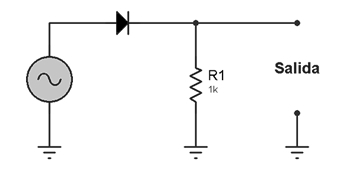
\includegraphics[width=0.47\textwidth]{images/4-4-1-circuito-rectificador-media-onda.jpg}
	\medskip
	\caption{Circuito rectificador de media onda.}
\end{figure}
\bigskip\bigskip


	Utilizando una señal de $10V_{pp}$ y 100Hz a la entrada, junto con una resistencia de 1$k\Omega$ y un diodo de silicio, se obtuvo a la salida una señal rectificada como la que se muestra en la \textit{Figura XX}. Esta última tiene una amplitud de 9,27V. Puede observarse que la señal de salida comienza a aumentar su amplitud a partir de los 0V unos instantes mas tarde que la señal de entrada. Este hecho se debe a que la tensión umbral del diodo de silicio es de 0,7V, es decir, hasta que no haya una caída mayor o igual a este valor sobre el diodo, este mismo no permitirá el paso de corriente. Por otro lado, la señal de salida posee una amplitud máxima menor a los 10V (aproximadamente 0,7V por debajo de esta), ya que parte de la tensión de la señal de entrada cae sobre el diodo.
\bigskip


\newpage
% Figura XX
\begin{figure}[h]
	\centering
	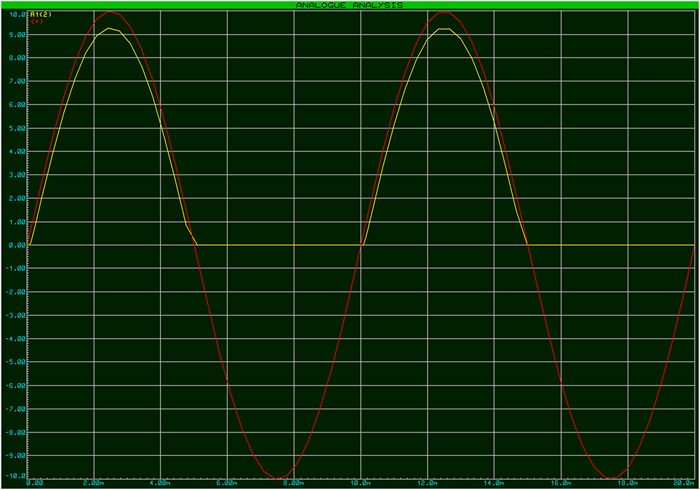
\includegraphics[width=0.95\textwidth]{images/4-4-2-grafico-circuito-rectificador-media-onda.jpg}
	\medskip
	\caption{Gráfico de la señal de salida de un rectificador\\ de media onda.}
\end{figure}
\bigskip\bigskip

	
	Agreguemos ahora a este circuito un capacitor de $20\mu F$ en paralelo a la resistencia que se encuentra previa a la salida, tal como se muestra en la \textit{Figura XXX}.
\bigskip


% Figura XXX
\begin{figure}[h]
	\centering
	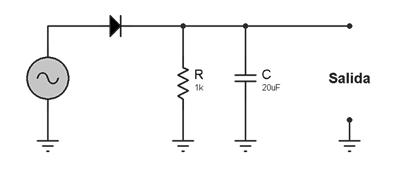
\includegraphics[width=0.54\textwidth]{images/4-4-3-circuito-rectificador-media-onda-con-filtro.jpg}
	\medskip
	\caption{Circuito rectificador de media onda con capacitor.}
\end{figure}
\bigskip\bigskip


	Al hacer esto, obtenemos sobre la salida la señal que se muestra en la \textit{Figura XXXX}, en la cual se puede observar que la tensión se mantiene entre dos valores acotados, lo que denomina \textit{ripple}. Es el capacitor el responsable de generar este comportamiento al cargarse en los tramos crecientes del semiciclo positivo de la señal de entrada y al descargarse en los instantes restantes (siendo fundamental que no llegue a descargarse por completo). Para este caso, el valor pico a pico de la tensión de ripple es de 3.08V, el cual resulta de la diferencia del máximo y mínimo valor de ripple. Cabe mencionar que cuanto menor sea este ripple, más grado de continuidad tendrá nuestra señal a la salida, por lo que podemos considerar que será mejor el rectificador.
\bigskip


\newpage
% Figura XXXX
\begin{figure}[h]
	\centering
	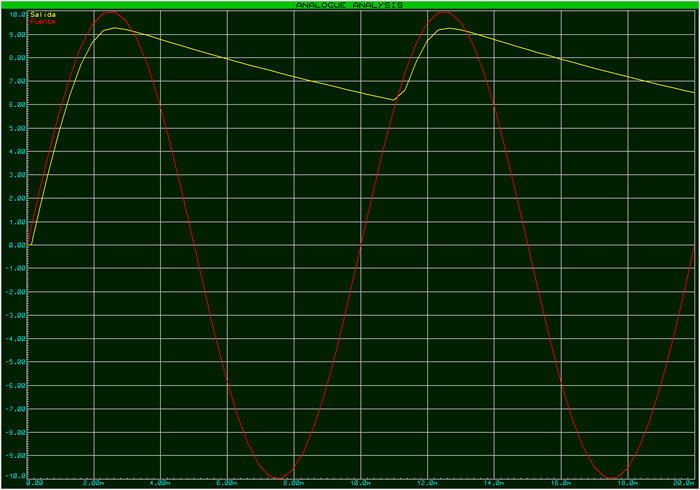
\includegraphics[width=0.95\textwidth]{images/4-4-4-grafico-circuito-rectificador-media-onda-con-filtro.jpg}
	\medskip
	\caption{Gráfico de la señal de salida de un rectificador\\ de media onda con capacitor.}
\end{figure}
\bigskip\bigskip


	Ahora, en la \textit{Figura XXXXX} se muestra el circuito rectificador conocido como \textit{rectificador de onda completa}. A diferencia del rectificador de media onda, en este caso, se utilizan los dos semiciclos  de la señal de entrada para rectificar.
\bigskip\bigskip
	

% Figura XXXXX
\begin{figure}[h]
	\centering
	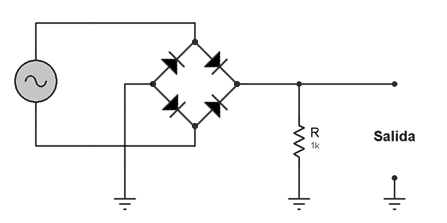
\includegraphics[width=0.60\textwidth]{images/4-4-5-circuito-rectificador-onda-completa.jpg}
	\medskip
	\caption{Circuito rectificador de onda completa.}
\end{figure}
\bigskip\bigskip


	Aplicando nuevamente una señal de $10V_{pp}$ y 100Hz a la entrada, junto con una resistencia de 1$k\Omega$ y un puente de diodos de silicio, se obtuvo a la salida una señal rectificada como la que se muestra en la \textit{Figura XXXXXX}. Esta última tiene una amplitud de 8,56V. Nótese que esta se encuentra 1,4V por debajo de los 10V de la señal de entrada, debiéndose esto a que se produce una caída de tensión sobre los dos diodos que se encuentran en directa en cada semiciclo de la señal. 
\bigskip


\newpage
% Figura XXXXXX
\begin{figure}[h]
	\centering
	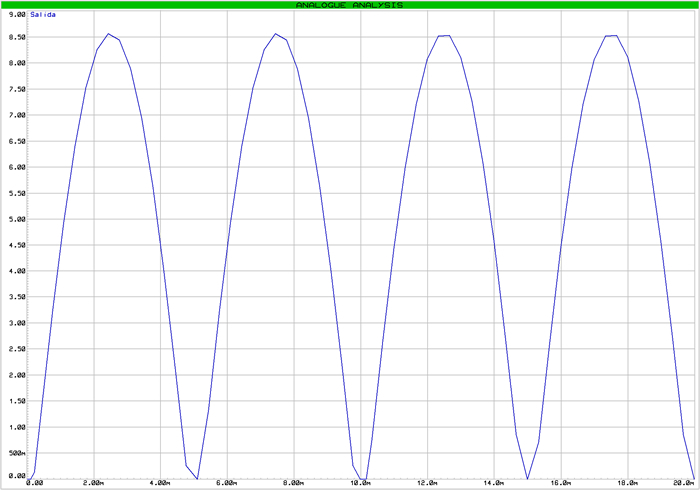
\includegraphics[width=0.95\textwidth]{images/4-4-6-grafico-circuito-rectificador-onda-completa.jpg}
	\medskip
	\caption{Gráfico de la señal de salida de un rectificador\\ de onda completa.}
\end{figure}
\bigskip\bigskip


	Acoplémosle a este circuito un capacitor de $10\mu F$ en paralelo a la resistencia que se encuentra previa a la salida, tal como se muestra en la \textit{Figura XXXXXXX}.
\bigskip


% Figura XXXXXXX
\begin{figure}[h]
	\centering
	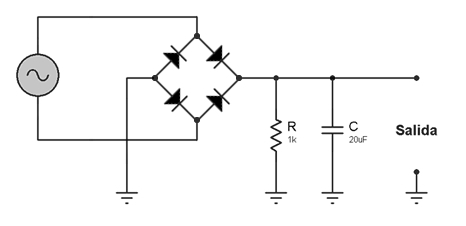
\includegraphics[width=0.633\textwidth]{images/4-4-7-circuito-rectificador-onda-completa-con-filtro.jpg}
	\medskip
	\caption{Circuito rectificador de onda completa con capacitor.}
\end{figure}
\bigskip\bigskip


Al hacer esto, sobre la salida obtenemos la señal que se muestra en \textit{Figura XXXXXXXX}, en la cual se puede observar que nuevamente se produce un ripple, pero que en este caso, el capacitor se carga y descarga dos veces por ciclo completo de la señal. Por último, se puede ver fácilmente que el valor pico a pico de la tensión de ripple es de 2,33V.


\newpage
% Figura XXXXXXXX
\begin{figure}[h]
	\centering
	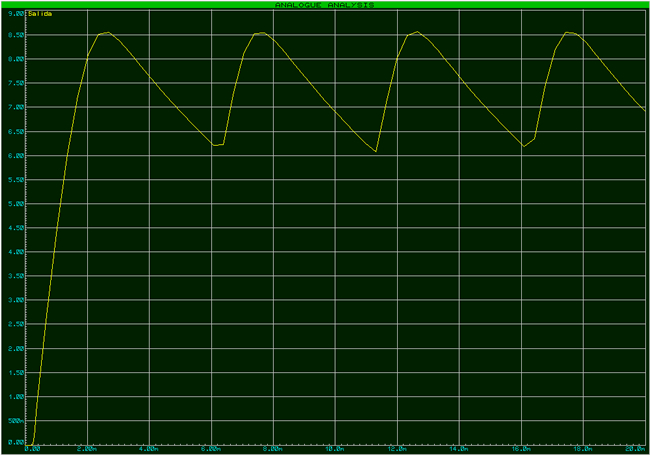
\includegraphics[width=0.88\textwidth]{images/4-4-8-grafico-circuito-rectificador-onda-completa-con-filtro.jpg}
	\medskip
	\caption{Gráfico de la señal de salida de un rectificador\\ de onda completa.}
\end{figure}
\bigskip\bigskip


	Por último, si modificamos el valor del capacitor, aumentando su capacidad a $50\mu F$, se obtiene la imagen de la \textit{Figura XXXXXXXXX}. Se puede observar claramente que con este aumento de la capacidad, el ripple disminuyó considerablemente a 0,6V. Esto se debe a que en este caso el capacitor va a poseer un tiempo de descarga mas extenso, provocando que la caída de tensión no sea de gran magnitud antes de que vuelva a darse el tramo en el que debe cargarse. 
\bigskip\bigskip


\newpage
% Figura XXXXXXXXX
\begin{figure}[h]
	\centering
	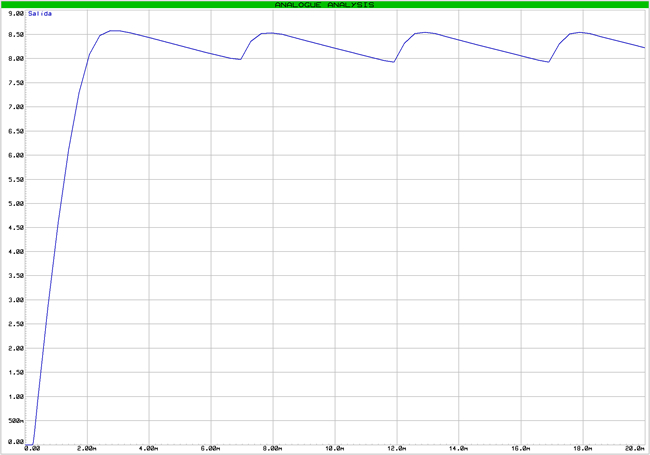
\includegraphics[width=0.88\textwidth]{images/4-4-9-grafico-circuito-rectificador-onda-completa-con-filtro-alt.jpg}
	\medskip
	\caption{Gráfico de la señal de salida de un rectificador\\ de onda completa.}
\end{figure}
\bigskip\bigskip




% CONCLUSIONES
\section{Conclusiones}

	De acuerdo a los resultados obtenidos en apartados anteriores podemos concluir que el efecto de carga que introducen las puntas en circuitos RC puede ser considerable tanto usando la punta \textit{X1} como la \textit{X10}. Esto se confirma al ver que los tiempos de crecimiento de las señales eran apreciablemente distintos de los calculados analíticamente. Aún así se puede ver que la punta atenuadora \textit{X10} es la mejor opción para realizar el trabajo práctico. Al ser el capacitor de $68 pF$, no hay punta que mejore las medidas realizadas mucho más, porque hay que tener en cuenta la capacidad de entrada del osciloscopio, que no se puede despreciar. 
	\par
	Se pudo observar también la relación directa entre el ancho de banda de los circuitos con el tiempo de crecimiento, y los valores utilizados de resistencias y capacidades. 
	\par
	Finalmente analizamos la utilización de diodos como rectificadores de media onda y onda completa, pudiendo así deducir los factores de forma.
\bigskip\bigskip


\newpage \textit{}
\newpage



% APÉNDICE A
\newpage
\vspace*{4cm}
\begin{center}
	\textbf{\Huge{Apéndice A}} \\
	\bigskip\bigskip
	\Large{\textit{``Hojas de datos de instrumentos de medición''}}
\end{center}


\newpage \textit{}
\newpage

\end{document}
